\section{Piecewise-linear Model}

The first model in this chapter and also the first constructed model is the piecewise-linear model.
It has 4 linear branches and is defined as the map $x_{n+1} = f(x_n) \mod 1$ where the following set of equations defines $f$.

\begin{align}
	f(x) & = \begin{cases}
		         g(x)                                        & \text{ if } x < \frac{1}{2} \\
		         g\left(x - \frac{1}{2}\right) + \frac{1}{2} & \text{ else}
	         \end{cases} \label{equ:app.model.lin.f} \\
	g(x) & = \begin{cases}
		         g_L(x) = \alpha \cdot x + \beta            & \text{ if } x < \frac{1}{4} \\
		         g_R(x) = \alpha \cdot x - \frac{\alpha}{4} & \text{ else}
	         \end{cases} \label{equ:app.model.lin.g}
\end{align}

One can see that this model definition is a little different from the model definitions in the main part of the thesis.
For example, \Cref{equ:app.model.lin.g} also enforces the symmetry that is found in the original model in this model explicitly.
And \Cref{equ:app.model.lin.g} then breaks each half of the model function into two smaller parts.
One difference is that $\alpha$ influences the slope of all four branches and also influences the offset of the function $g_R$.
$g_R$ governs the branches $f_\B$ and $f_\D$ and its offset causes the branch $f_\B$ to start at $0$ and the branch $f_\D$ to start at $\frac{1}{2}$.

\begin{figure}
	\centering
	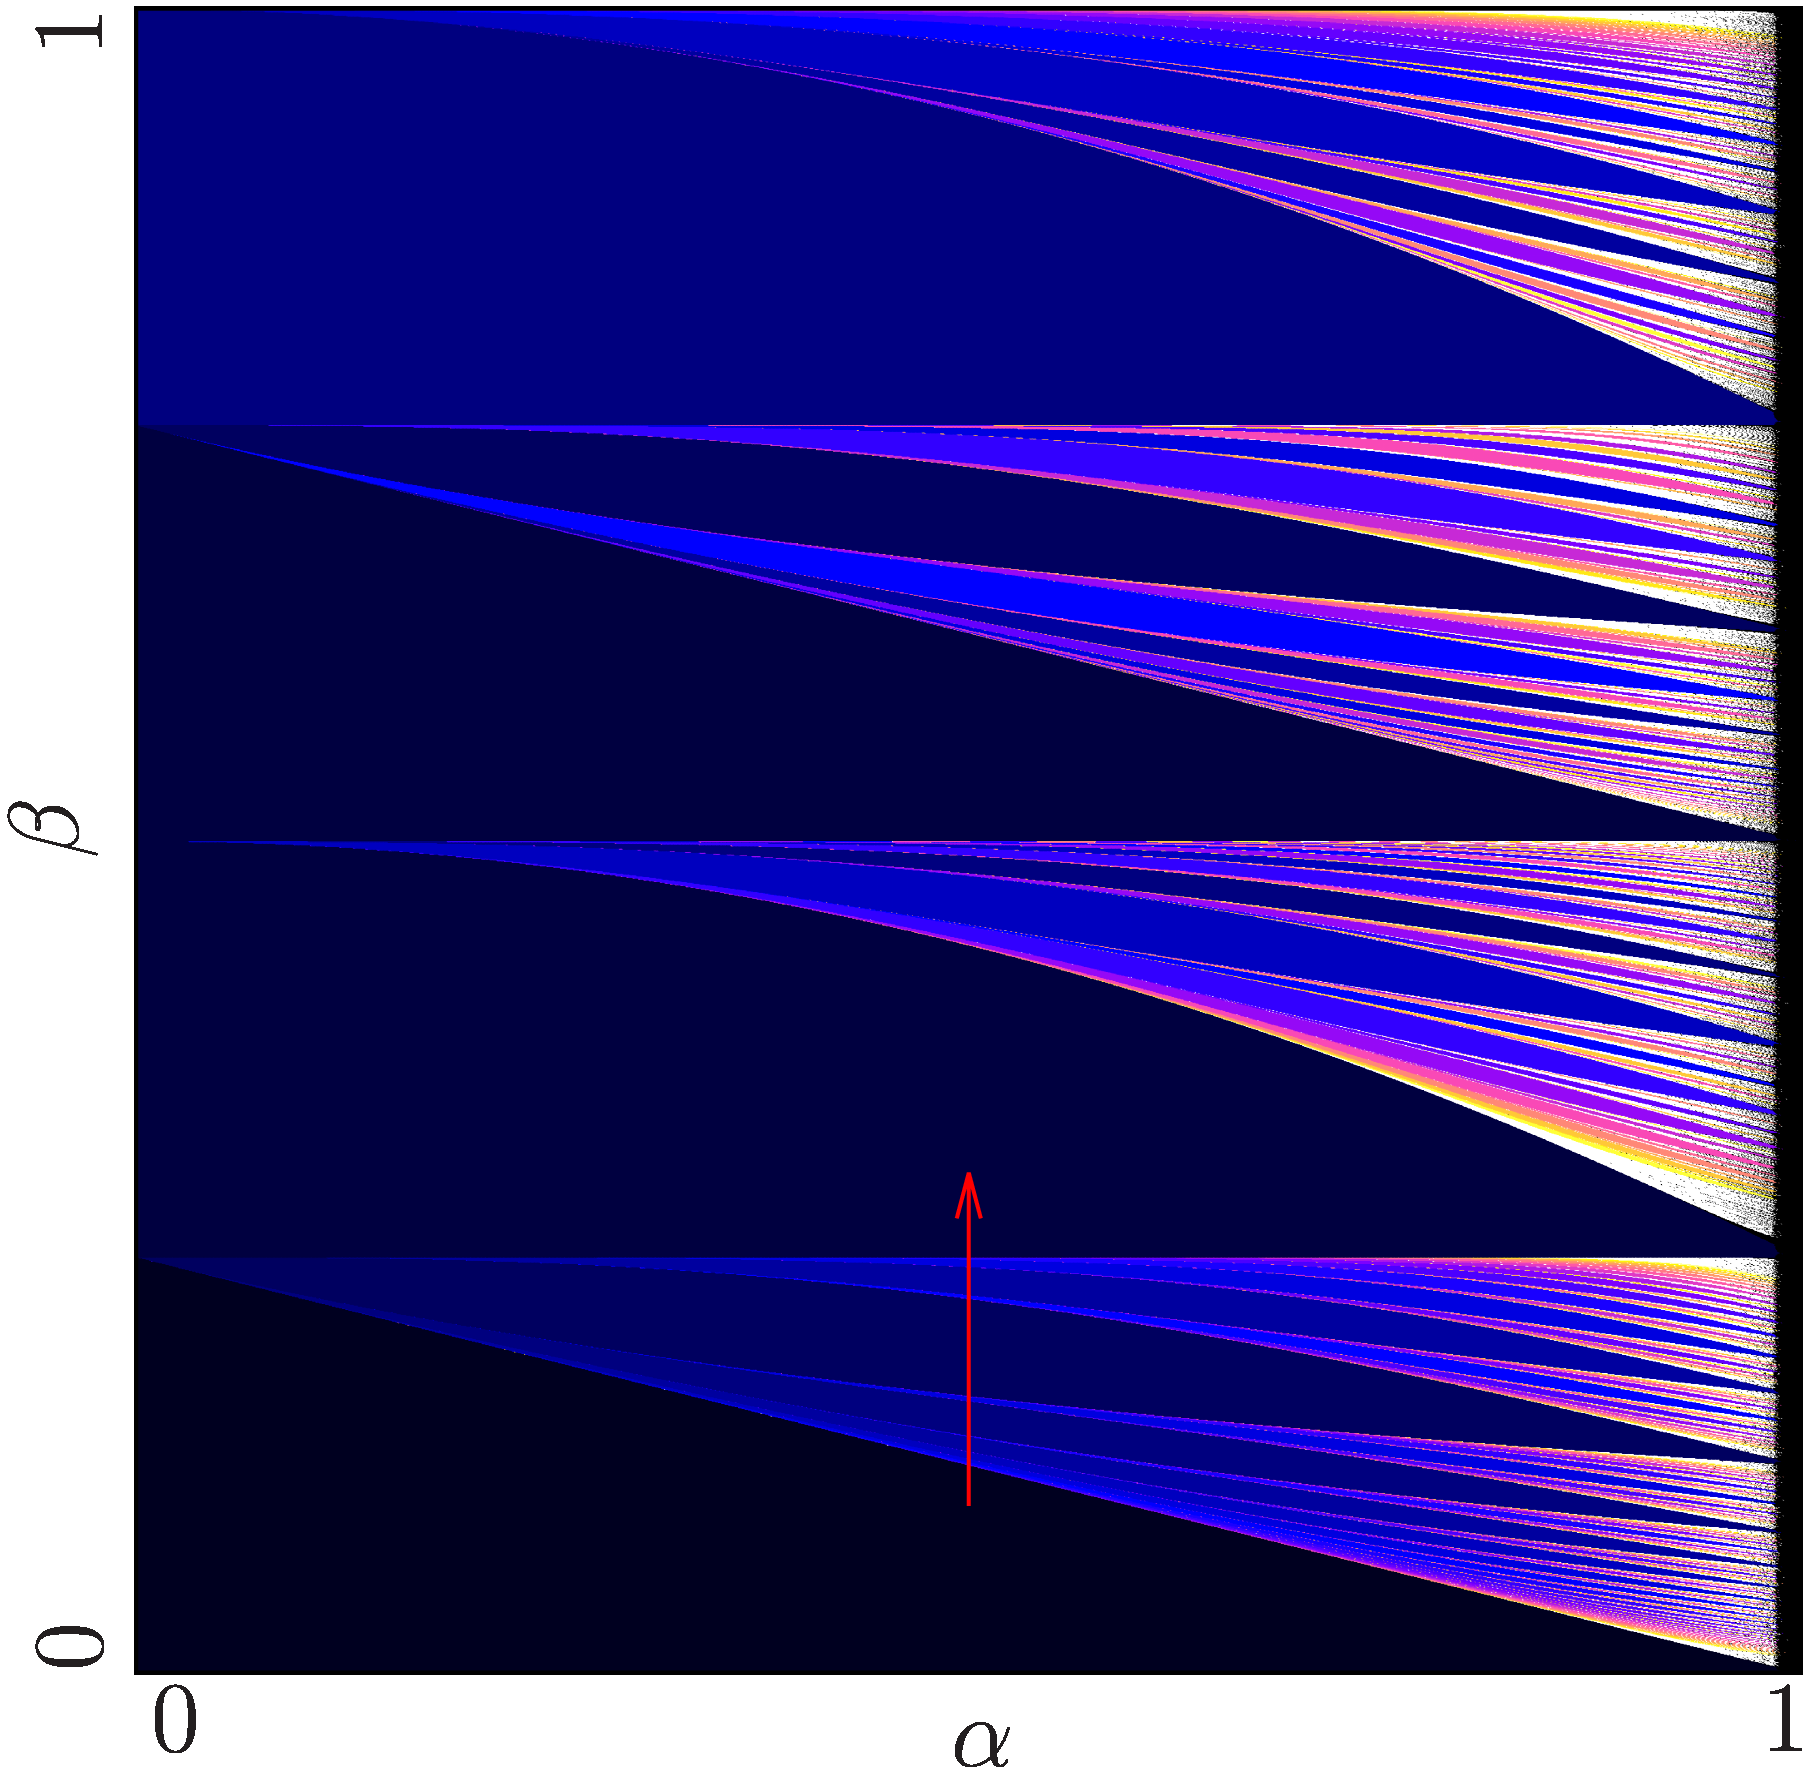
\includegraphics[width=0.7 \textwidth]{../Figures/A/A.1/result.png}
	\caption[2D scan of periods associated with parameter regions in the piecewise-linear model]{
		2D scan of periods associated with parameter regions in the piecewise-linear model.
		The red arrow marks the parameter range used for the 1D period scan in \Cref{fig:app.model.lin.1D}.
	}
	\label{fig:app.model.lin.2D}
\end{figure}

\begin{figure}
	\centering
	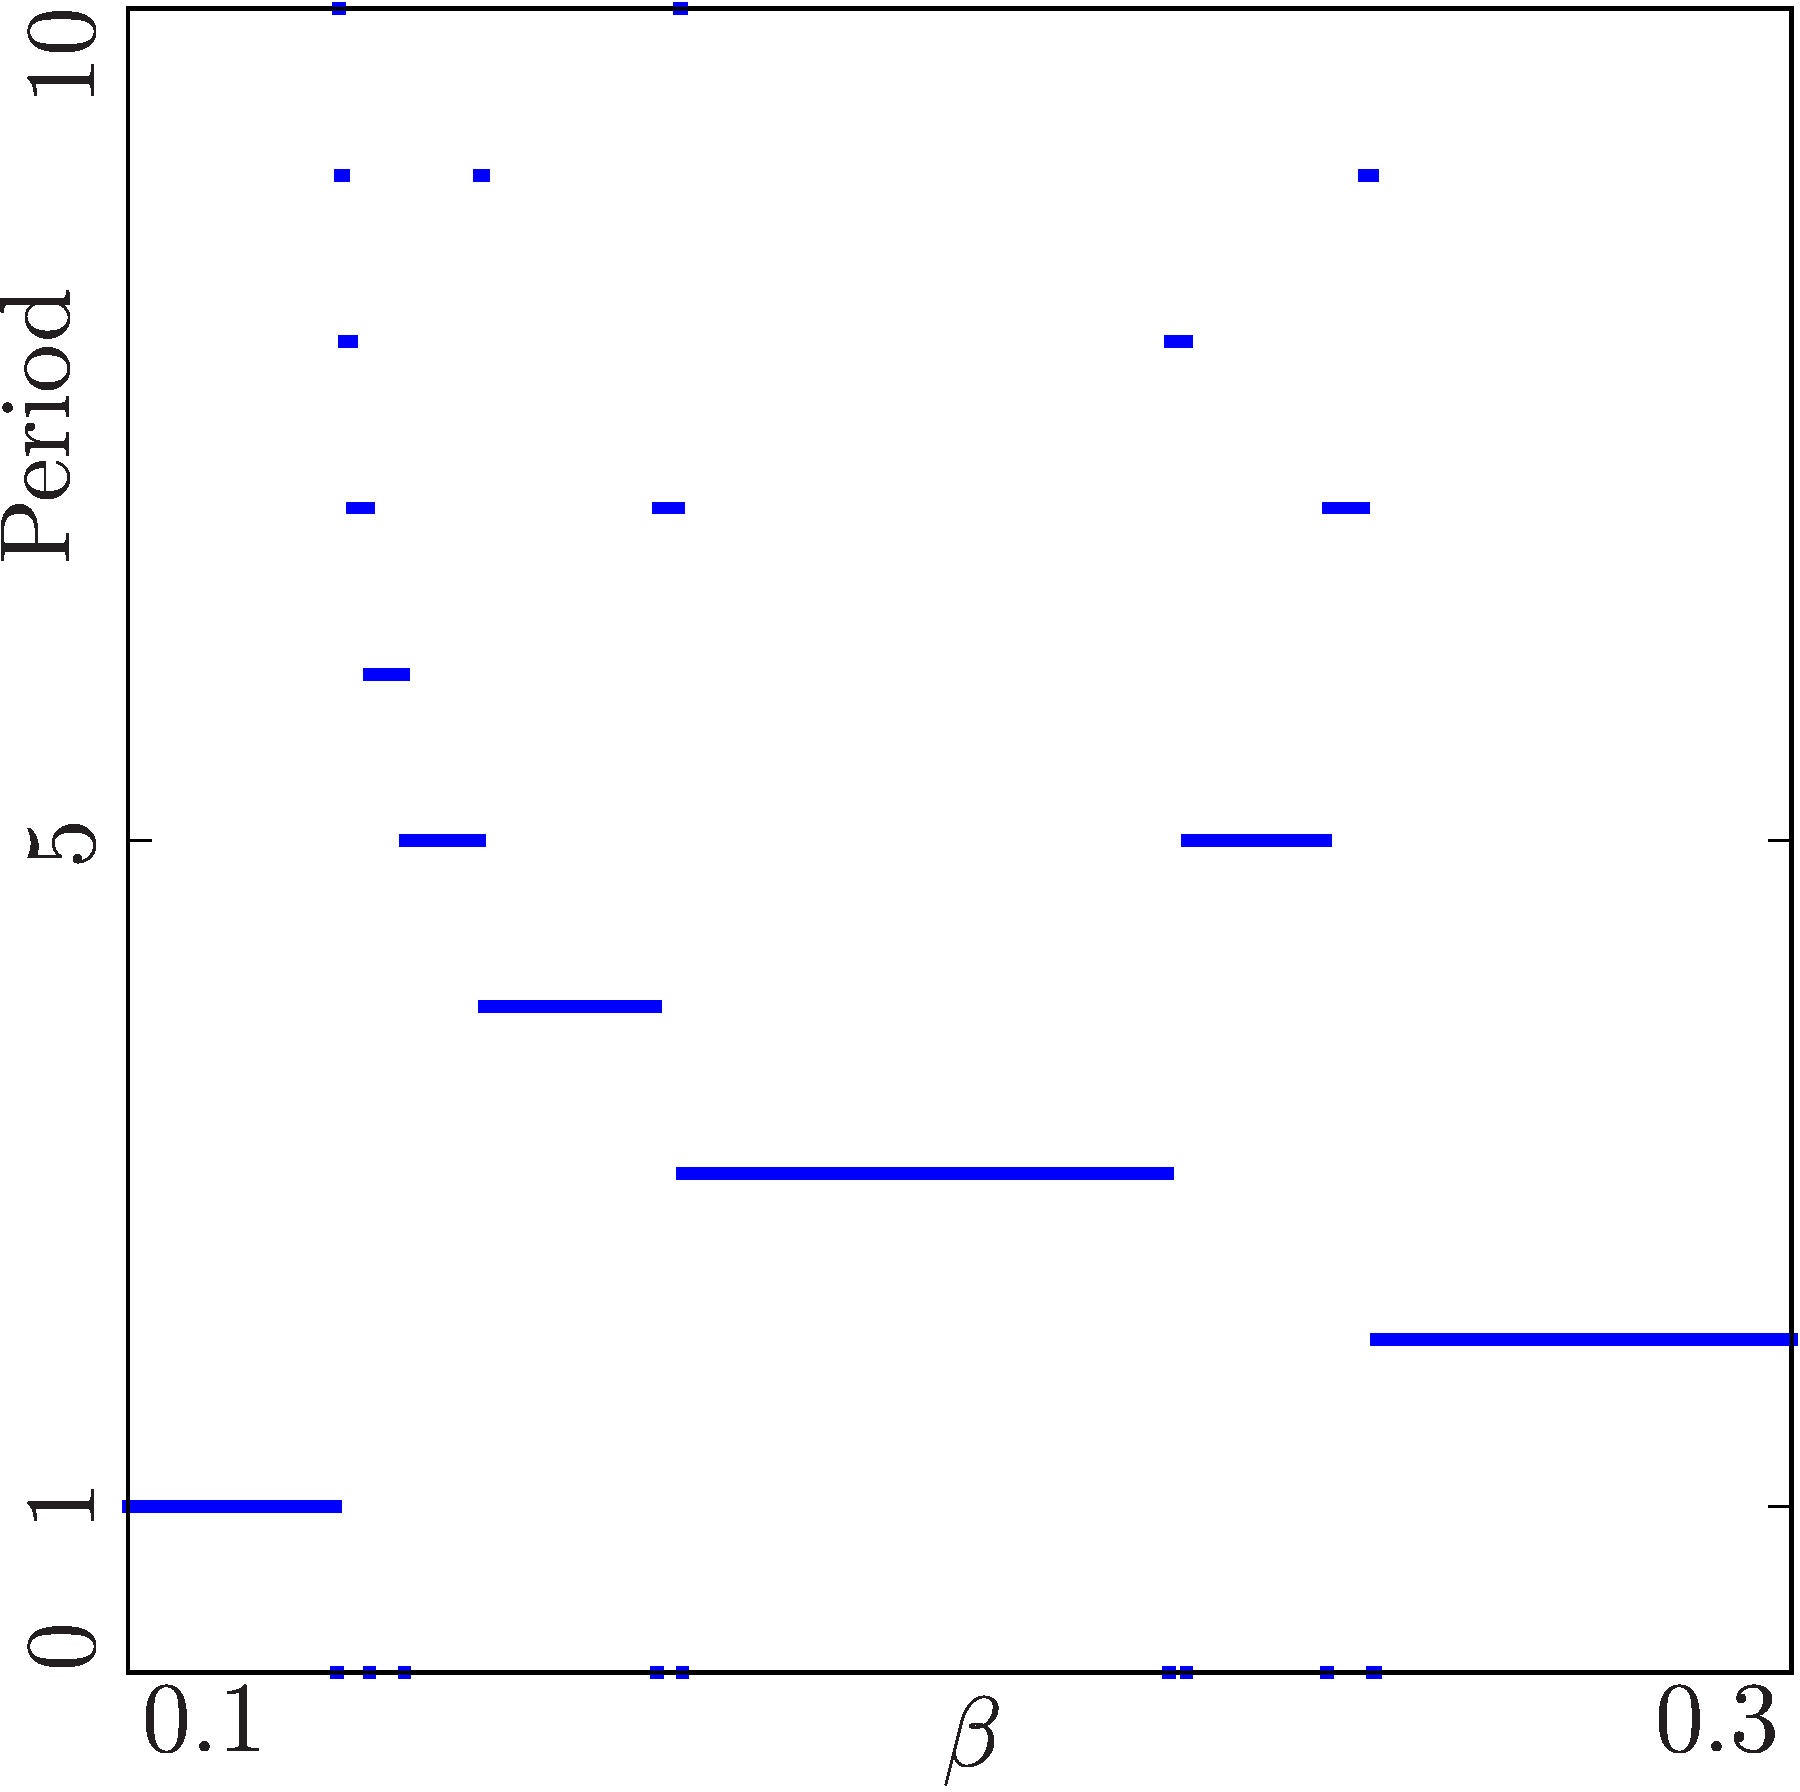
\includegraphics[width=0.6 \textwidth]{../Figures/A/A.2/result.png}
	\caption[1D scan of periods associated with parameter regions in the piecewise-linear model]{
		1D scan of periods associated with parameter regions in the piecewise-linear model.
		The parameter range is marked with a red arrow in \Cref{fig:app.model.lin.2D}.
	}
	\label{fig:app.model.lin.1D}
\end{figure}

\Cref{fig:app.model.lin.2D} shows a 2D scan of the periods associated with parameter regions in this model.
The structures look a lot like \gls{pa} structures.
Scanning the periods in 1D, results in \Cref{fig:app.model.lin.1D}.
This indeed shows a pattern that is typical for \gls{pa} structures.
